

\tikzset{every picture/.style={line width=0.75pt}} %set default line width to 0.75pt        

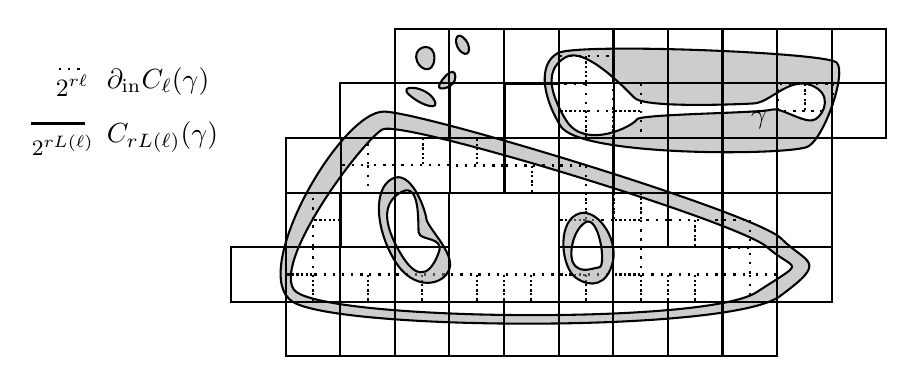
\begin{tikzpicture}[x=0.75pt,y=0.75pt,yscale=-1,xscale=1]
%uncomment if require: \path (0,215); %set diagram left start at 0, and has height of 215

%Shape: Polygon Curved [id:ds7719121712646727] 
\draw  [fill={rgb, 255:red, 155; green, 155; blue, 155 }  ,fill opacity=0.5 ] (318.38,65.52) .. controls (339.13,66.28) and (497.71,114.59) .. (509.69,126.74) .. controls (521.68,138.88) and (533.2,136.85) .. (508.77,154.56) .. controls (484.34,172.27) and (295.79,171) .. (274.13,157.09) .. controls (252.46,143.18) and (297.64,64.77) .. (318.38,65.52) -- cycle ;
%Shape: Polygon Curved [id:ds45748805954474026] 
\draw  [fill={rgb, 255:red, 255; green, 255; blue, 255 }  ,fill opacity=1 ] (317.46,74.12) .. controls (326.68,69.07) and (488.95,118.64) .. (502.78,130.78) .. controls (516.61,142.92) and (522.6,136.35) .. (497.71,152.54) .. controls (472.81,168.72) and (283.81,166.19) .. (274.59,151.02) .. controls (269.66,142.9) and (279.64,122.9) .. (291.4,105.28) .. controls (301.62,89.98) and (313.18,76.48) .. (317.46,74.12) -- cycle ;
%Shape: Polygon Curved [id:ds6204914078619962] 
\draw  [fill={rgb, 255:red, 155; green, 155; blue, 155 }  ,fill opacity=0.5 ] (401.93,37.35) .. controls (411.15,32.29) and (531.39,36.97) .. (536.32,41.9) .. controls (541.25,46.83) and (530.4,78.07) .. (522.51,82.35) .. controls (514.62,86.62) and (412.47,87.61) .. (403.25,72.43) .. controls (394.03,57.25) and (392.71,42.41) .. (401.93,37.35) -- cycle ;
%Shape: Polygon Curved [id:ds485406802439853] 
\draw  [fill={rgb, 255:red, 255; green, 255; blue, 255 }  ,fill opacity=1 ] (405.88,39.23) .. controls (415.1,34.17) and (434.05,54.01) .. (438.98,58.95) .. controls (443.91,63.88) and (488.53,62.02) .. (496.42,61.58) .. controls (504.31,61.14) and (513.3,48.81) .. (523.82,52.75) .. controls (534.35,56.7) and (530.73,66.24) .. (526.12,69.2) .. controls (521.52,72.16) and (509.35,62.95) .. (504.75,64.59) .. controls (500.15,66.24) and (440.91,66.64) .. (439.97,69.31) .. controls (439.03,71.97) and (415.1,84.76) .. (405.88,69.58) .. controls (396.66,54.41) and (396.66,44.29) .. (405.88,39.23) -- cycle ;
%Straight Lines [id:da2906575942901778] 
\draw  [dash pattern={on 0.84pt off 2.51pt}]  (161.51,45.08) -- (174.66,45.08) ;
%Shape: Polygon [id:ds9469171879037334] 
\draw  [dash pattern={on 0.84pt off 2.51pt}] (297.14,117.7) -- (297.14,130.85) -- (283.98,130.85) -- (283.98,117.7) -- cycle ;
%Shape: Polygon [id:ds74802235265109] 
\draw  [dash pattern={on 0.84pt off 2.51pt}] (283.98,130.85) -- (283.98,144.01) -- (270.83,144.01) -- (270.83,130.85) -- cycle ;
%Shape: Polygon [id:ds3390238747929295] 
\draw  [dash pattern={on 0.84pt off 2.51pt}] (362.91,144.01) -- (362.91,157.16) -- (349.75,157.16) -- (349.75,144.01) -- cycle ;
%Shape: Polygon [id:ds6521339259740929] 
\draw  [dash pattern={on 0.84pt off 2.51pt}] (349.75,144.01) -- (349.75,157.16) -- (336.6,157.16) -- (336.6,144.01) -- cycle ;
%Shape: Polygon [id:ds6134588230692475] 
\draw  [dash pattern={on 0.84pt off 2.51pt}] (336.6,144.01) -- (336.6,157.16) -- (323.45,157.16) -- (323.45,144.01) -- cycle ;
%Shape: Polygon [id:ds8022486699311164] 
\draw  [dash pattern={on 0.84pt off 2.51pt}] (323.45,144.01) -- (323.45,157.16) -- (310.29,157.16) -- (310.29,144.01) -- cycle ;
%Shape: Polygon [id:ds3940441180216041] 
\draw  [dash pattern={on 0.84pt off 2.51pt}] (310.29,144.01) -- (310.29,157.16) -- (297.14,157.16) -- (297.14,144.01) -- cycle ;
%Shape: Polygon [id:ds885660205830769] 
\draw  [dash pattern={on 0.84pt off 2.51pt}] (297.14,144.01) -- (297.14,157.16) -- (283.98,157.16) -- (283.98,144.01) -- cycle ;
%Shape: Polygon [id:ds8141196508041333] 
\draw  [dash pattern={on 0.84pt off 2.51pt}] (283.98,144.01) -- (283.98,157.16) -- (270.83,157.16) -- (270.83,144.01) -- cycle ;
%Shape: Polygon [id:ds49902531580098897] 
\draw  [dash pattern={on 0.84pt off 2.51pt}] (468.14,144.01) -- (468.14,157.16) -- (454.98,157.16) -- (454.98,144.01) -- cycle ;
%Shape: Polygon [id:ds908380295656456] 
\draw  [dash pattern={on 0.84pt off 2.51pt}] (481.29,144.01) -- (481.29,157.16) -- (468.14,157.16) -- (468.14,144.01) -- cycle ;
%Shape: Polygon [id:ds7405486178508747] 
\draw  [dash pattern={on 0.84pt off 2.51pt}] (494.45,144.01) -- (494.45,157.16) -- (481.29,157.16) -- (481.29,144.01) -- cycle ;
%Shape: Polygon [id:ds4666989377312746] 
\draw  [dash pattern={on 0.84pt off 2.51pt}] (507.6,130.85) -- (507.6,144.01) -- (494.45,144.01) -- (494.45,130.85) -- cycle ;
%Shape: Polygon [id:ds5043807343630617] 
\draw  [dash pattern={on 0.84pt off 2.51pt}] (494.45,117.92) -- (494.45,131.07) -- (481.29,131.07) -- (481.29,117.92) -- cycle ;
%Shape: Polygon [id:ds46740228807508455] 
\draw  [dash pattern={on 0.84pt off 2.51pt}] (481.29,117.7) -- (481.29,130.85) -- (468.14,130.85) -- (468.14,117.7) -- cycle ;
%Shape: Polygon [id:ds057863749533867304] 
\draw  [dash pattern={on 0.84pt off 2.51pt}] (468.14,117.7) -- (468.14,130.85) -- (454.98,130.85) -- (454.98,117.7) -- cycle ;
%Shape: Polygon [id:ds45904169950816365] 
\draw  [dash pattern={on 0.84pt off 2.51pt}] (454.98,104.55) -- (454.98,117.7) -- (441.83,117.7) -- (441.83,104.55) -- cycle ;
%Shape: Polygon [id:ds27162019148811367] 
\draw  [dash pattern={on 0.84pt off 2.51pt}] (441.94,104.66) -- (441.94,117.81) -- (428.79,117.81) -- (428.79,104.66) -- cycle ;
%Shape: Polygon [id:ds19254570149483718] 
\draw  [dash pattern={on 0.84pt off 2.51pt}] (428.79,104.66) -- (428.79,117.81) -- (415.63,117.81) -- (415.63,104.66) -- cycle ;
%Shape: Polygon [id:ds49728361026253387] 
\draw  [dash pattern={on 0.84pt off 2.51pt}] (415.63,91.5) -- (415.63,104.66) -- (402.48,104.66) -- (402.48,91.5) -- cycle ;
%Shape: Polygon [id:ds9084345807697809] 
\draw  [dash pattern={on 0.84pt off 2.51pt}] (402.48,91.5) -- (402.48,104.66) -- (389.32,104.66) -- (389.32,91.5) -- cycle ;
%Shape: Polygon [id:ds5760638963961741] 
\draw  [dash pattern={on 0.84pt off 2.51pt}] (389.32,91.5) -- (389.32,104.66) -- (376.17,104.66) -- (376.17,91.5) -- cycle ;
%Shape: Polygon [id:ds7199116926860121] 
\draw  [dash pattern={on 0.84pt off 2.51pt}] (376.17,78.35) -- (376.17,91.5) -- (363.02,91.5) -- (363.02,78.35) -- cycle ;
%Shape: Polygon [id:ds18537435892924714] 
\draw  [dash pattern={on 0.84pt off 2.51pt}] (363.02,78.35) -- (363.02,91.5) -- (349.86,91.5) -- (349.86,78.35) -- cycle ;
%Shape: Polygon [id:ds2684210616160845] 
\draw  [dash pattern={on 0.84pt off 2.51pt}] (349.97,78.24) -- (349.97,91.39) -- (336.82,91.39) -- (336.82,78.24) -- cycle ;
%Shape: Polygon [id:ds1359811707669788] 
\draw  [dash pattern={on 0.84pt off 2.51pt}] (336.82,78.24) -- (336.82,91.39) -- (323.66,91.39) -- (323.66,78.24) -- cycle ;
%Shape: Polygon [id:ds20903983953703853] 
\draw  [dash pattern={on 0.84pt off 2.51pt}] (323.66,78.24) -- (323.66,91.39) -- (310.51,91.39) -- (310.51,78.24) -- cycle ;
%Shape: Polygon [id:ds6016840181460674] 
\draw  [dash pattern={on 0.84pt off 2.51pt}] (310.51,91.39) -- (310.51,104.55) -- (297.36,104.55) -- (297.36,91.39) -- cycle ;
%Shape: Polygon [id:ds24315613042930928] 
\draw  [dash pattern={on 0.84pt off 2.51pt}] (297.36,104.55) -- (297.36,117.7) -- (284.2,117.7) -- (284.2,104.55) -- cycle ;
%Shape: Polygon [id:ds44288283804591555] 
\draw  [dash pattern={on 0.84pt off 2.51pt}] (441.83,51.93) -- (441.83,65.08) -- (428.68,65.08) -- (428.68,51.93) -- cycle ;
%Shape: Polygon [id:ds29140353468656566] 
\draw  [dash pattern={on 0.84pt off 2.51pt}] (441.83,65.08) -- (441.83,78.24) -- (428.68,78.24) -- (428.68,65.08) -- cycle ;
%Shape: Polygon [id:ds5738976445859719] 
\draw  [dash pattern={on 0.84pt off 2.51pt}] (428.68,65.08) -- (428.68,78.24) -- (415.52,78.24) -- (415.52,65.08) -- cycle ;
%Shape: Polygon [id:ds9458615119554507] 
\draw  [dash pattern={on 0.84pt off 2.51pt}] (415.52,65.08) -- (415.52,78.24) -- (402.37,78.24) -- (402.37,65.08) -- cycle ;
%Shape: Polygon [id:ds9556331805799785] 
\draw  [dash pattern={on 0.84pt off 2.51pt}] (415.63,130.96) -- (415.63,144.12) -- (402.48,144.12) -- (402.48,130.96) -- cycle ;
%Shape: Polygon [id:ds07078227648534274] 
\draw  [dash pattern={on 0.84pt off 2.51pt}] (415.63,117.81) -- (415.63,130.96) -- (402.48,130.96) -- (402.48,117.81) -- cycle ;
%Shape: Polygon [id:ds5318529403076371] 
\draw  [dash pattern={on 0.84pt off 2.51pt}] (415.63,104.66) -- (415.63,117.81) -- (402.48,117.81) -- (402.48,104.66) -- cycle ;
%Shape: Polygon [id:ds3724527045642546] 
\draw  [dash pattern={on 0.84pt off 2.51pt}] (441.83,117.7) -- (441.83,130.85) -- (428.68,130.85) -- (428.68,117.7) -- cycle ;
%Shape: Polygon [id:ds6537714920979174] 
\draw  [dash pattern={on 0.84pt off 2.51pt}] (441.83,130.85) -- (441.83,144.01) -- (428.68,144.01) -- (428.68,130.85) -- cycle ;
%Shape: Polygon [id:ds01841907862367964] 
\draw  [dash pattern={on 0.84pt off 2.51pt}] (376.06,144.01) -- (376.06,157.16) -- (362.91,157.16) -- (362.91,144.01) -- cycle ;
%Shape: Polygon [id:ds9168510976965855] 
\draw  [dash pattern={on 0.84pt off 2.51pt}] (389.21,144.01) -- (389.21,157.16) -- (376.06,157.16) -- (376.06,144.01) -- cycle ;
%Shape: Polygon [id:ds133752889376058] 
\draw  [dash pattern={on 0.84pt off 2.51pt}] (402.37,144.01) -- (402.37,157.16) -- (389.21,157.16) -- (389.21,144.01) -- cycle ;
%Shape: Polygon [id:ds5445607576226932] 
\draw  [dash pattern={on 0.84pt off 2.51pt}] (415.52,144.01) -- (415.52,157.16) -- (402.37,157.16) -- (402.37,144.01) -- cycle ;
%Shape: Polygon [id:ds4710742525873627] 
\draw  [dash pattern={on 0.84pt off 2.51pt}] (428.68,144.01) -- (428.68,157.16) -- (415.52,157.16) -- (415.52,144.01) -- cycle ;
%Shape: Polygon [id:ds0993394639113866] 
\draw  [dash pattern={on 0.84pt off 2.51pt}] (441.83,144.01) -- (441.83,157.16) -- (428.68,157.16) -- (428.68,144.01) -- cycle ;
%Shape: Polygon [id:ds9688662207235097] 
\draw  [dash pattern={on 0.84pt off 2.51pt}] (454.98,144.01) -- (454.98,157.16) -- (441.83,157.16) -- (441.83,144.01) -- cycle ;
%Shape: Polygon [id:ds8635232874486733] 
\draw  [dash pattern={on 0.84pt off 2.51pt}] (534.35,52.15) -- (534.35,65.3) -- (521.19,65.3) -- (521.19,52.15) -- cycle ;
%Shape: Polygon [id:ds5474312516527738] 
\draw  [dash pattern={on 0.84pt off 2.51pt}] (521.19,52.15) -- (521.19,65.3) -- (508.04,65.3) -- (508.04,52.15) -- cycle ;
%Shape: Polygon [id:ds0882763981081287] 
\draw  [dash pattern={on 0.84pt off 2.51pt}] (415.48,38.92) -- (415.48,52.07) -- (402.32,52.07) -- (402.32,38.92) -- cycle ;
%Shape: Polygon [id:ds5863956636612095] 
\draw  [dash pattern={on 0.84pt off 2.51pt}] (415.59,51.88) -- (415.59,65.04) -- (402.43,65.04) -- (402.43,51.88) -- cycle ;
%Shape: Polygon [id:ds3374241862659888] 
\draw  [dash pattern={on 0.84pt off 2.51pt}] (428.74,38.73) -- (428.74,51.88) -- (415.59,51.88) -- (415.59,38.73) -- cycle ;
%Shape: Polygon Curved [id:ds3136063643108614] 
\draw  [fill={rgb, 255:red, 155; green, 155; blue, 155 }  ,fill opacity=0.5 ] (322.02,97.91) .. controls (331.24,92.85) and (338.15,112.83) .. (338.61,117.13) .. controls (339.07,121.43) and (352.44,133.57) .. (349.68,141.41) .. controls (346.91,149.26) and (332.62,152.54) .. (323.4,137.37) .. controls (314.18,122.19) and (312.8,102.97) .. (322.02,97.91) -- cycle ;
%Shape: Polygon Curved [id:ds8592435053982214] 
\draw  [fill={rgb, 255:red, 255; green, 255; blue, 255 }  ,fill opacity=1 ] (326.63,104.23) .. controls (335.85,99.17) and (334.46,119.41) .. (334.92,123.71) .. controls (335.39,128.01) and (347.37,125.48) .. (344.61,133.32) .. controls (341.84,141.16) and (335.85,149.76) .. (326.63,134.58) .. controls (317.41,119.41) and (317.41,109.29) .. (326.63,104.23) -- cycle ;
%Shape: Polygon Curved [id:ds907592743570509] 
\draw  [fill={rgb, 255:red, 155; green, 155; blue, 155 }  ,fill opacity=0.5 ] (410.71,115.26) .. controls (419.93,110.2) and (431.22,126.29) .. (428.46,137.92) .. controls (425.69,149.56) and (417.63,150.42) .. (410.71,145.61) .. controls (403.8,140.81) and (401.49,120.32) .. (410.71,115.26) -- cycle ;
%Shape: Polygon Curved [id:ds03767156835124452] 
\draw  [fill={rgb, 255:red, 255; green, 255; blue, 255 }  ,fill opacity=1 ] (415.3,118.85) .. controls (421.76,115.06) and (425.57,140.05) .. (421.88,140.56) .. controls (418.19,141.06) and (413.94,143.34) .. (410.25,139.8) .. controls (406.56,136.26) and (408.85,122.65) .. (415.3,118.85) -- cycle ;
%Shape: Polygon Curved [id:ds37847618736103883] 
\draw  [fill={rgb, 255:red, 155; green, 155; blue, 155 }  ,fill opacity=0.5 ] (342.46,40.08) .. controls (341.99,48.43) and (334.16,45.14) .. (333.7,39.32) .. controls (333.24,33.51) and (342.92,31.73) .. (342.46,40.08) -- cycle ;
%Shape: Polygon Curved [id:ds33089979622692933] 
\draw  [fill={rgb, 255:red, 155; green, 155; blue, 155 }  ,fill opacity=0.5 ] (330.47,57.53) .. controls (336.46,62.85) and (346.14,65.63) .. (341.99,59.31) .. controls (337.85,52.98) and (324.48,52.22) .. (330.47,57.53) -- cycle ;
%Shape: Polygon Curved [id:ds5704837252533028] 
\draw  [fill={rgb, 255:red, 155; green, 155; blue, 155 }  ,fill opacity=0.5 ] (352.6,48.43) .. controls (353.06,53.99) and (343.84,56.02) .. (344.76,52.98) .. controls (345.68,49.95) and (352.14,42.86) .. (352.6,48.43) -- cycle ;
%Shape: Polygon Curved [id:ds6662816043413571] 
\draw  [fill={rgb, 255:red, 155; green, 155; blue, 155 }  ,fill opacity=0.5 ] (356.28,29.71) .. controls (352.14,26.42) and (351.67,34.26) .. (355.82,37.05) .. controls (359.97,39.83) and (360.43,33) .. (356.28,29.71) -- cycle ;
%Straight Lines [id:da8324164530924741] 
\draw    (148.05,71.24) -- (174.14,71.24) ;
%Shape: Rectangle [id:dp016281378285771364] 
\draw   (270.83,130.85) -- (297.14,130.85) -- (297.14,157.16) -- (270.83,157.16) -- cycle ;
%Shape: Rectangle [id:dp031187767199392535] 
\draw   (402.37,157.16) -- (428.68,157.16) -- (428.68,183.47) -- (402.37,183.47) -- cycle ;
%Shape: Rectangle [id:dp7439595771566538] 
\draw   (376.06,157.16) -- (402.37,157.16) -- (402.37,183.47) -- (376.06,183.47) -- cycle ;
%Shape: Rectangle [id:dp21081262299581116] 
\draw   (349.75,157.16) -- (376.06,157.16) -- (376.06,183.47) -- (349.75,183.47) -- cycle ;
%Shape: Rectangle [id:dp9979902356877028] 
\draw   (323.45,157.16) -- (349.75,157.16) -- (349.75,183.47) -- (323.45,183.47) -- cycle ;
%Shape: Rectangle [id:dp25500254709091363] 
\draw   (297.14,157.16) -- (323.45,157.16) -- (323.45,183.47) -- (297.14,183.47) -- cycle ;
%Shape: Rectangle [id:dp31813557414436944] 
\draw   (271.05,104.55) -- (297.36,104.55) -- (297.36,130.85) -- (271.05,130.85) -- cycle ;
%Shape: Rectangle [id:dp5079179805357779] 
\draw   (244.52,130.85) -- (270.83,130.85) -- (270.83,157.16) -- (244.52,157.16) -- cycle ;
%Shape: Rectangle [id:dp06484125368769633] 
\draw   (428.68,104.55) -- (454.98,104.55) -- (454.98,130.85) -- (428.68,130.85) -- cycle ;
%Shape: Rectangle [id:dp73161761517393] 
\draw   (376.28,78.24) -- (402.59,78.24) -- (402.59,104.55) -- (376.28,104.55) -- cycle ;
%Shape: Rectangle [id:dp3067282552401762] 
\draw   (349.75,51.93) -- (376.06,51.93) -- (376.06,78.24) -- (349.75,78.24) -- cycle ;
%Shape: Rectangle [id:dp6253342239026325] 
\draw   (402.59,78.24) -- (428.9,78.24) -- (428.9,104.55) -- (402.59,104.55) -- cycle ;
%Shape: Rectangle [id:dp2516566363815891] 
\draw   (454.98,104.55) -- (481.29,104.55) -- (481.29,130.85) -- (454.98,130.85) -- cycle ;
%Shape: Rectangle [id:dp33859379981551996] 
\draw   (481.29,104.55) -- (507.6,104.55) -- (507.6,130.85) -- (481.29,130.85) -- cycle ;
%Shape: Rectangle [id:dp08675172167266276] 
\draw   (481.29,130.85) -- (507.6,130.85) -- (507.6,157.16) -- (481.29,157.16) -- cycle ;
%Shape: Rectangle [id:dp6309115889257129] 
\draw   (481.29,157.16) -- (507.6,157.16) -- (507.6,183.47) -- (481.29,183.47) -- cycle ;
%Shape: Rectangle [id:dp1957246245635238] 
\draw   (507.6,130.85) -- (533.91,130.85) -- (533.91,157.16) -- (507.6,157.16) -- cycle ;
%Shape: Rectangle [id:dp4121080799743302] 
\draw   (454.98,157.16) -- (481.29,157.16) -- (481.29,183.47) -- (454.98,183.47) -- cycle ;
%Shape: Rectangle [id:dp08010298979753405] 
\draw   (428.68,157.16) -- (454.98,157.16) -- (454.98,183.47) -- (428.68,183.47) -- cycle ;
%Shape: Rectangle [id:dp1252765805240872] 
\draw   (376.28,51.93) -- (402.59,51.93) -- (402.59,78.24) -- (376.28,78.24) -- cycle ;
%Shape: Rectangle [id:dp010546433583140002] 
\draw   (297.14,130.85) -- (323.45,130.85) -- (323.45,157.16) -- (297.14,157.16) -- cycle ;
%Shape: Rectangle [id:dp30472645935671516] 
\draw   (270.83,157.16) -- (297.14,157.16) -- (297.14,183.47) -- (270.83,183.47) -- cycle ;
%Shape: Rectangle [id:dp8529586322125453] 
\draw   (323.45,130.85) -- (349.75,130.85) -- (349.75,157.16) -- (323.45,157.16) -- cycle ;
%Shape: Rectangle [id:dp8963181776703018] 
\draw   (297.14,104.55) -- (323.45,104.55) -- (323.45,130.85) -- (297.14,130.85) -- cycle ;
%Shape: Rectangle [id:dp7650056909586043] 
\draw   (507.6,51.93) -- (533.91,51.93) -- (533.91,78.24) -- (507.6,78.24) -- cycle ;
%Shape: Rectangle [id:dp737838398824495] 
\draw   (349.75,25.62) -- (376.06,25.62) -- (376.06,51.93) -- (349.75,51.93) -- cycle ;
%Shape: Rectangle [id:dp40359134910784555] 
\draw   (271.05,78.24) -- (297.36,78.24) -- (297.36,104.55) -- (271.05,104.55) -- cycle ;
%Shape: Rectangle [id:dp026875721677431574] 
\draw   (323.45,104.55) -- (349.75,104.55) -- (349.75,130.85) -- (323.45,130.85) -- cycle ;
%Shape: Rectangle [id:dp31425516474546256] 
\draw   (297.36,78.24) -- (323.66,78.24) -- (323.66,104.55) -- (297.36,104.55) -- cycle ;
%Shape: Rectangle [id:dp28470585560506145] 
\draw   (349.97,78.24) -- (376.28,78.24) -- (376.28,104.55) -- (349.97,104.55) -- cycle ;
%Shape: Rectangle [id:dp6634857522656132] 
\draw   (533.91,25.62) -- (560.22,25.62) -- (560.22,51.93) -- (533.91,51.93) -- cycle ;
%Shape: Rectangle [id:dp6240416675837892] 
\draw   (402.37,130.85) -- (428.68,130.85) -- (428.68,157.16) -- (402.37,157.16) -- cycle ;
%Shape: Rectangle [id:dp3926273505770723] 
\draw   (402.37,104.55) -- (428.68,104.55) -- (428.68,130.85) -- (402.37,130.85) -- cycle ;
%Shape: Rectangle [id:dp5689309753936915] 
\draw   (402.59,51.93) -- (428.9,51.93) -- (428.9,78.24) -- (402.59,78.24) -- cycle ;
%Shape: Rectangle [id:dp0656735074870558] 
\draw   (402.59,25.62) -- (428.9,25.62) -- (428.9,51.93) -- (402.59,51.93) -- cycle ;
%Shape: Rectangle [id:dp5659467788220274] 
\draw   (376.02,25.77) -- (402.32,25.77) -- (402.32,52.07) -- (376.02,52.07) -- cycle ;
%Shape: Rectangle [id:dp2322857995349199] 
\draw   (428.68,78.24) -- (454.98,78.24) -- (454.98,104.55) -- (428.68,104.55) -- cycle ;
%Shape: Rectangle [id:dp5950494352002125] 
\draw   (507.6,104.55) -- (533.91,104.55) -- (533.91,130.85) -- (507.6,130.85) -- cycle ;
%Shape: Rectangle [id:dp06642002570282668] 
\draw   (297.14,51.93) -- (323.45,51.93) -- (323.45,78.24) -- (297.14,78.24) -- cycle ;
%Shape: Rectangle [id:dp8927582871077535] 
\draw   (323.45,25.62) -- (349.75,25.62) -- (349.75,51.93) -- (323.45,51.93) -- cycle ;
%Shape: Rectangle [id:dp5865471281069827] 
\draw   (323.66,51.93) -- (349.97,51.93) -- (349.97,78.24) -- (323.66,78.24) -- cycle ;
%Shape: Rectangle [id:dp040276194507303575] 
\draw   (533.91,51.93) -- (560.22,51.93) -- (560.22,78.24) -- (533.91,78.24) -- cycle ;
%Shape: Rectangle [id:dp3794607755206678] 
\draw   (481.29,25.62) -- (507.6,25.62) -- (507.6,51.93) -- (481.29,51.93) -- cycle ;
%Shape: Rectangle [id:dp9599180213474743] 
\draw   (455.2,25.62) -- (481.51,25.62) -- (481.51,51.93) -- (455.2,51.93) -- cycle ;
%Shape: Rectangle [id:dp18179124416522785] 
\draw   (454.98,51.93) -- (481.29,51.93) -- (481.29,78.24) -- (454.98,78.24) -- cycle ;
%Shape: Rectangle [id:dp8798012541309046] 
\draw   (454.98,78.24) -- (481.29,78.24) -- (481.29,104.55) -- (454.98,104.55) -- cycle ;
%Shape: Rectangle [id:dp34660091038270013] 
\draw   (428.9,51.93) -- (455.2,51.93) -- (455.2,78.24) -- (428.9,78.24) -- cycle ;
%Shape: Rectangle [id:dp25002765157464313] 
\draw   (428.74,25.58) -- (455.05,25.58) -- (455.05,51.88) -- (428.74,51.88) -- cycle ;
%Shape: Rectangle [id:dp582307469904453] 
\draw   (507.6,25.62) -- (533.91,25.62) -- (533.91,51.93) -- (507.6,51.93) -- cycle ;
%Shape: Rectangle [id:dp7452503714467449] 
\draw   (481.29,51.93) -- (507.6,51.93) -- (507.6,78.24) -- (481.29,78.24) -- cycle ;
%Shape: Rectangle [id:dp6648668143658343] 
\draw   (481.29,78.24) -- (507.6,78.24) -- (507.6,104.55) -- (481.29,104.55) -- cycle ;
%Shape: Rectangle [id:dp731030687311671] 
\draw   (507.6,78.24) -- (533.91,78.24) -- (533.91,104.55) -- (507.6,104.55) -- cycle ;

% Text Node
\draw (183.24,42.84) node [anchor=north west][inner sep=0.75pt]    {$\partial _{\mathrm{in}}\mathfrak{C}_{\ell }( \gamma )$};
% Text Node
\draw (158.57,46.14) node [anchor=north west][inner sep=0.75pt]  [font=\small]  {$2^{r\ell }$};
% Text Node
\draw (493.59,63.84) node [anchor=north west][inner sep=0.75pt]    {$\gamma $};
% Text Node
\draw (147.04,75.24) node [anchor=north west][inner sep=0.75pt]  [font=\footnotesize]  {$2^{rL( \ell )}$};
% Text Node
\draw (183.24,68.95) node [anchor=north west][inner sep=0.75pt]    {$\mathscr{C}_{rL( \ell )}( \gamma )$};


\end{tikzpicture}